\documentclass{paper}


\usepackage[utf8]{inputenc}



\usepackage[english]{babel}
\usepackage[a4paper, margin=0.8in]{geometry}

\usepackage{parskip}

\usepackage{amsthm}
\usepackage{amssymb}
\usepackage{amsmath}


\usepackage{graphicx} 

% variables you can adjust
\newcommand{\titleVar}{\large Seminar Report on\\ \LARGE TCUDB: Accelerating Database with Tensor Processors \\{\large {by Yu-Ching Hu, Yuliang Li, Hung-Wei Tseng}}
}

\newcommand{\authorVar}{David Raphael Zollikofer}
% end variables you can adjust


% last configuration before document starts
\title{\titleVar}
\author{David Raphael Zollikofer\\ ETH Zürich}
\date{\today}



\usepackage{mathpazo}

% optional math environments



\begin{document}
	
\twocolumn[\maketitle 
\hrule 

\begin{abstract}Recent advances in hardware accelerators for matrix multiplications have massively sped up deep learning workflows in the past. In this seminar report we will outline how NVIDIAs Tensor Cores can be used to sped up database workloads; for this we will take a close look at the framework presented in \cite{hu2021tcudb}, analyze it, compare it to other relevant literature \cite{he2022query}. Last but not least we will also highlight shortcomings of the presented approaches and give a short outlook.
\end{abstract}

\hrule\bigskip
]

	

\section{Introduction}
The introduction of Tensor Cores for NVIDIA GPUs has enable significant speed improvements for deep learning workflows. As these tensor cores speed up matrix multiplication workloads there is a keen interest in speeding up other workloads. The paper "Accelerating Database with Tensor Processors" by Yu-Ching Hu, Yuliang Li, Hung-Wei Tseng \cite{hu2021tcudb} presents an interesting framework to use Tensor Cores for database acceleration. For this they introduce a new mapping from database operators to tensor operations which allows them to ....
	
	\section{Using Tensor Cores to Accelerate Databases}
	
	\subsection{The Tensor Abstraction}
	Databases must be able to represent a wide variety of data types. Matrixmultiplication, the very thing the Tensor Core can accelerate 
	
	limited precision too 
	
	
	
	\subsection{Mapping Database Operators to Tensor Operations}
	
	\subsection{End-to-End Pipeline}
	

	\begin{figure}
		\centering
		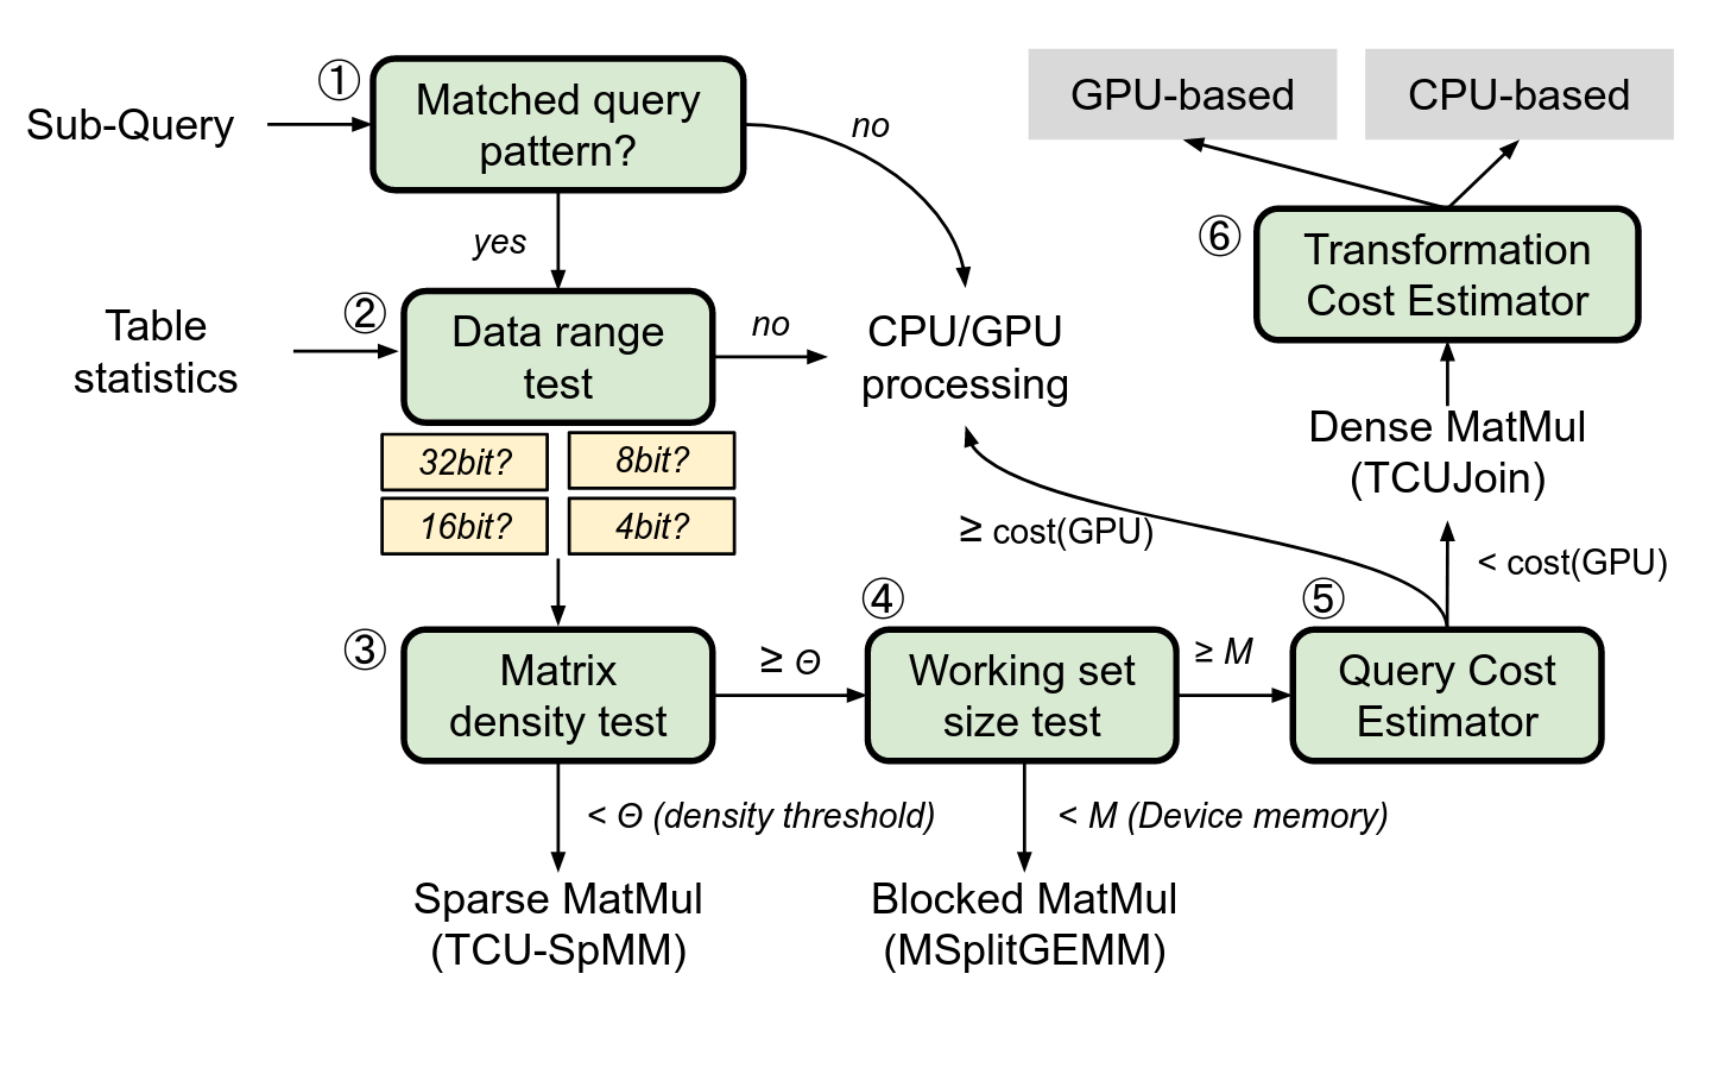
\includegraphics[width=1\linewidth]{pipeline}
		\caption{The workflow of the TCUDB query optimizer. Figure from \cite{hu2021tcudb}.}
		\label{fig:pipeline}
	\end{figure}
	
	
	\section{Comparison to Related Work}
	As tensor processors are quite a new development there is little other literature to compare the "Accelerating Database with Tensor Processors" paper to. 
	
	There is ample previous work on accelerating database workloads with other specialized hardware such as (CITE HERE) which uses NVIDIA CUDA cores for database acceleration.
	
	Another approach which utilizes NVIDIA Tensor Cores is "Query Processing on Tensor Computation Runtimes" by He et al. which ...
	
	CUDA 
	\cite{he2022query}lol \cite{hu2021tcudb}
	  \cite{sun_2022}
	if we use tensors we must use 
	
	\section{Performance Evaluation}
	
	clearly good on ...
	
	very expected
	
	\section{Shortcomings}
	
	monetDB is super old, why not compared to Vectorwise, questionable 
	
	TPC-H benchmark like others
	
	clearly inefficient? 
	
	how many runs, average?
	
	
	\section{Conclusion}
	
\bibliographystyle{plain}
\bibliography{bibliography}
	

\end{document}
